\documentclass[presentation]{subfiles}

\onlyinsubfile{
\usepackage[citestyle=numeric,backend=bibtex]{biblatex}
\bibliography{references}
  % \beamertemplategridbackground[1mm]
}


\begin{document}

\section{Complexity}

\begin{frame}{Complexity}
  What kinds of problems do we mean when we talk about complexity?
  \begin{itemize}
    \item<1-> Can crowds help you write something?\\
    \scriptsize{
      \textcite{bernsteinSoylent,Kim:2014:CSI:2556288.2556986,Nebeling:2016:WCW:2858036.2858169}
    }
    \item<2-> Can crowds critique novel designs?\\
    \scriptsize{
      \textcite{yuanAlmost,fuge2014analysis}
    }
    \item<3-> Can crowds create things from whole cloth?\\
    \scriptsize{
      \textcite{KimStoria,Kim2017,Hahn:2016:KAB:2858036.2858364,Lasecki:2014:LSR:2661334.2661352}
    }
  \end{itemize}
\end{frame}


\begin{frame}{What does the crowdsourcing literature say?}
\begin{columns}
  \begin{column}{0.6\textwidth}
    \begin{itemize}
      \item Build complexity into the process
      \begin{itemize}
        \item<1> Apply CS methods to people\\
        \scriptsize{
          \textcite{crowdForgeKittur}
        }
        \item<2> Humans as computational units\\
        \scriptsize{
          \textcite{Lasecki:2014:LSR:2661334.2661352}
        }
        \item<3> Crowdsourcing workflows as function state machines\\
        \scriptsize{\textcite{latoza2014microtask}
        }
      \end{itemize}
    \end{itemize}
  \end{column}
  
  \begin{column}{0.4\textwidth}
    \begin{figure}
    \only<1>{
    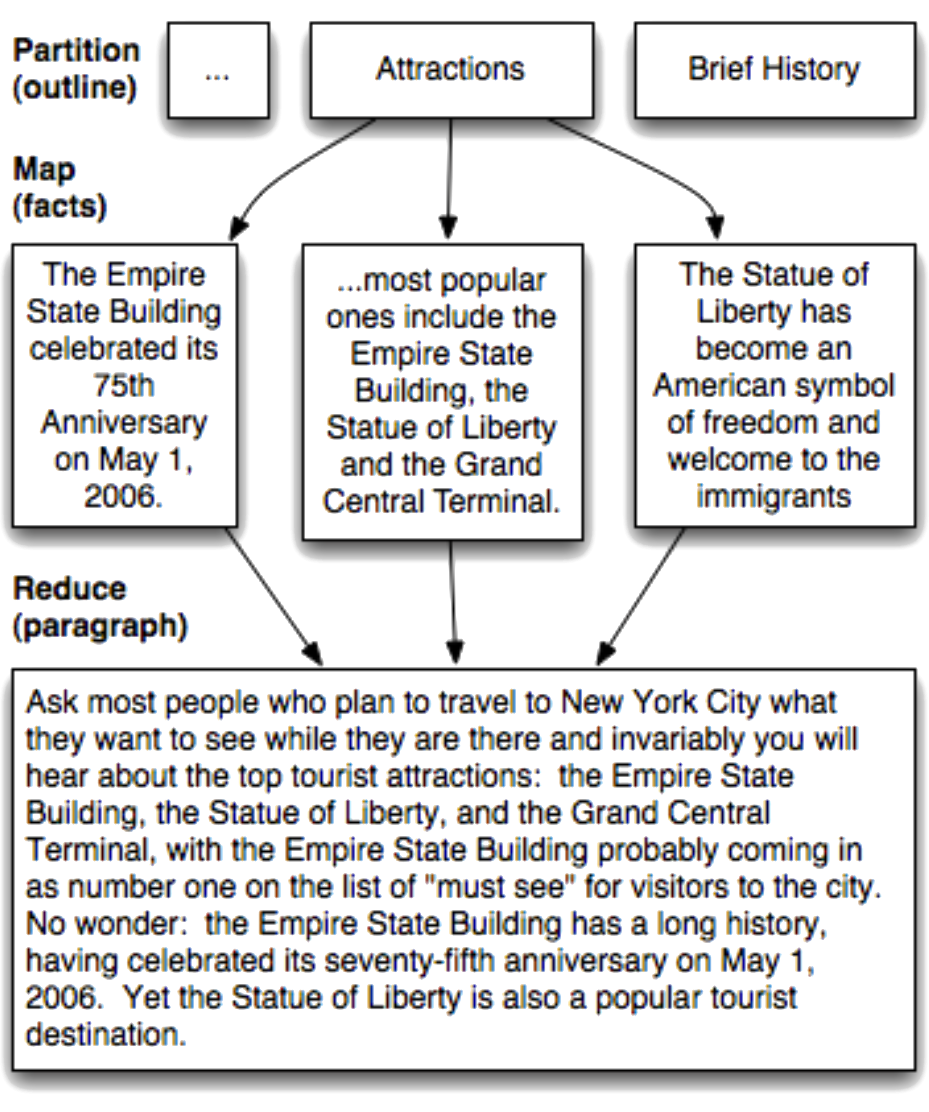
\includegraphics[width=\textwidth]{figures/complexity/cw_literature/mapReduce.png}
    }
    
    \only<2>{
      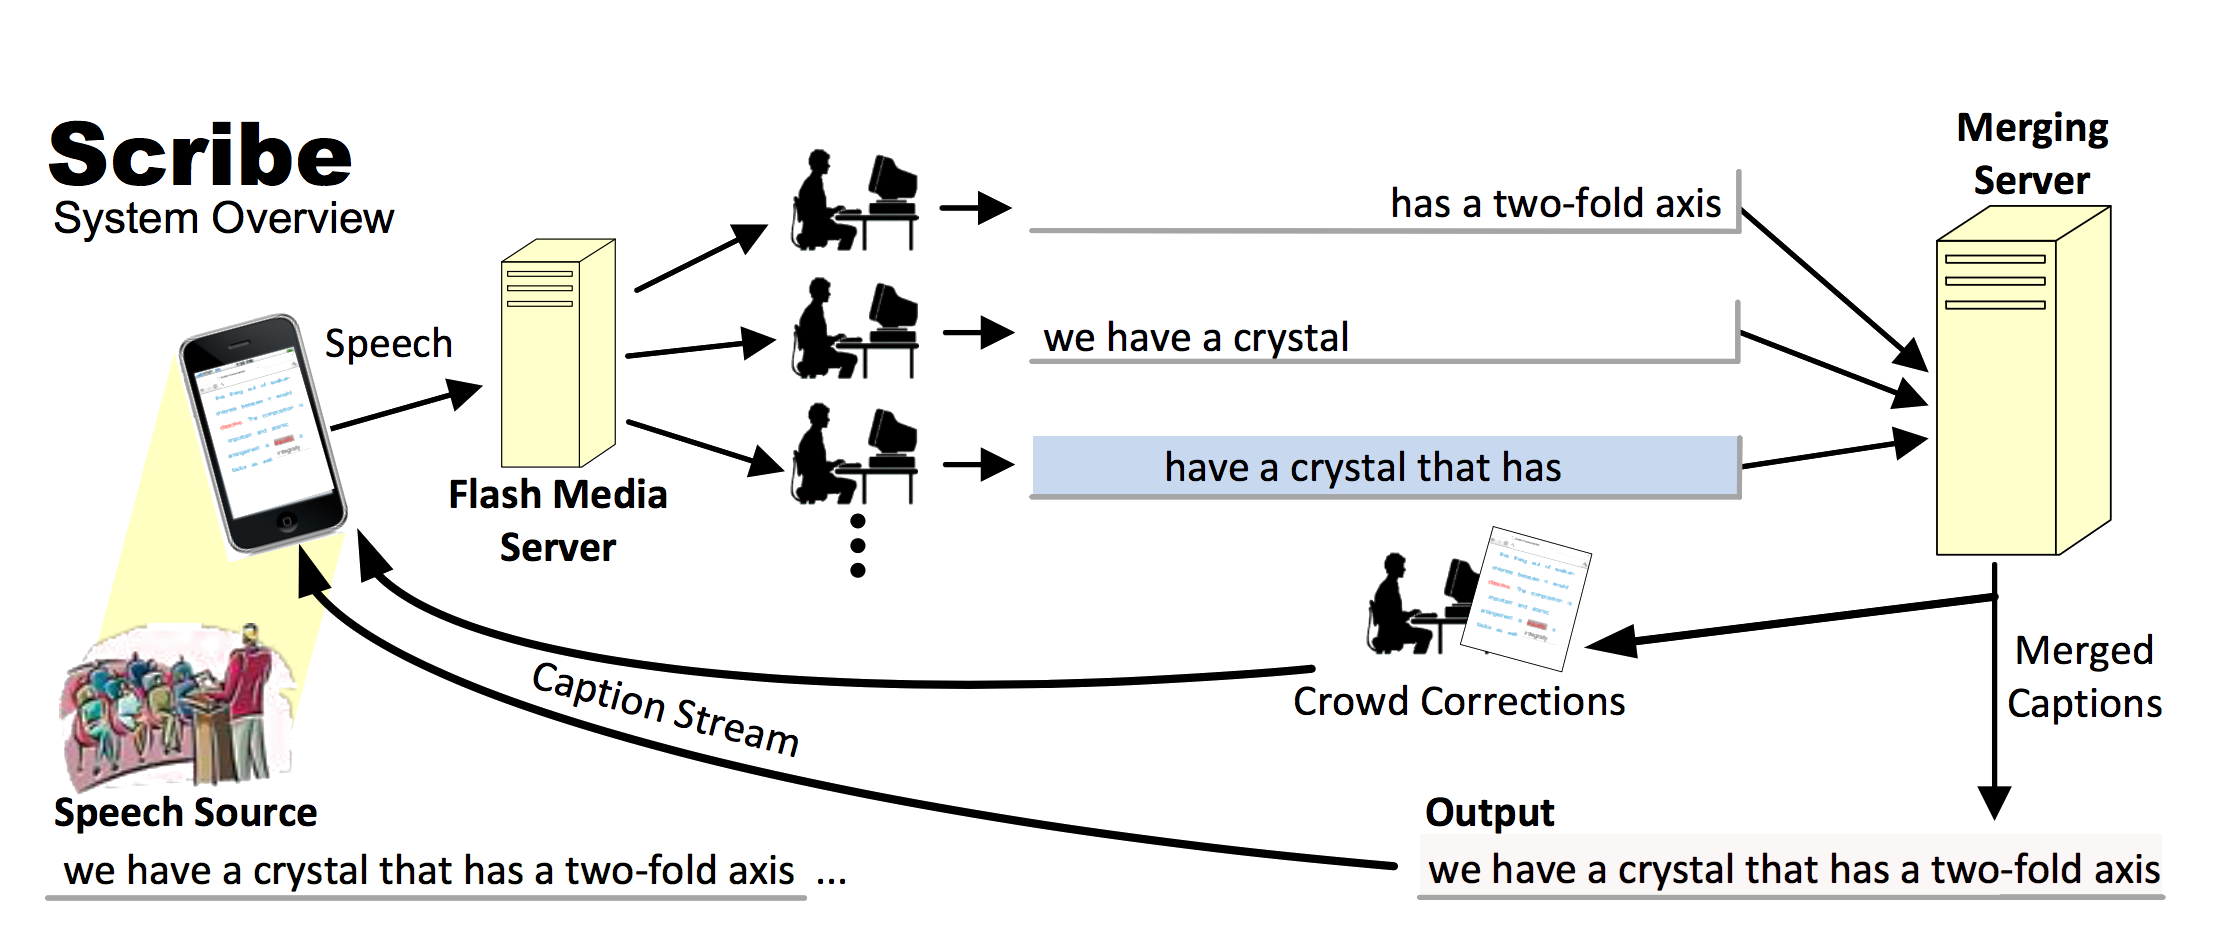
\includegraphics[width=\textwidth]{figures/complexity/cw_literature/scribe.png}
    }
    \only<3>{
      \begin{adjustbox}{max totalsize={\textwidth}{\textheight},center}
      \begin{tikzpicture}[->,>=stealth',auto, node distance=4cm,
                          thick,transform shape]
        \node[state,label=above:{Described}]                       (A)                    {};
        \node[state,label=left:{Described written}]                (B) [below of=A]       {};
        \node[state,label=left:{Run Tests}]                        (D) [below of=B]       {};
        \node[state,label=below:{Described written buggy}]         (C) [below right of=D] {};
        \node[state,label=below:{Described written buggy}]         (E) [below left of=D]  {};

        \path[every node/.style={sloped,anchor=south}]
              (A) edge              node {Write description} (B)
              (B) edge [loop right] node {Edit code} (B)
                  edge              node {Edit code} (D)
              (D) edge              node {} (C)
                  edge              node {} (E)
              (C) edge [bend right] node {Debug} (B)
                  edge [bend right] node {Debug} (D)
              (E) edge [bend right] node {Edit Code} (D)
                  edge [bend left]  node {Edit Code} (B);
        \end{tikzpicture}
        \end{adjustbox}
    }
    \end{figure}
  \end{column}
  
\end{columns}
\end{frame}

\begin{frame}{What does the piecework literature say?}
    % \begin{itemize}
      % \item
      George Airy (astronomer) used a very similar approach~\cite{grier2013computers}
      % \begin{itemize}
      %   \item Break work up so that individual tasks are simple\\
      %   Make the process \textit{itself} compile the final product.
      % \end{itemize}
    % \end{itemize}
    % \vspace{0mm}
    \begin{columns}
    \begin{column}{0.6\textwidth}
      \begin{figure}
        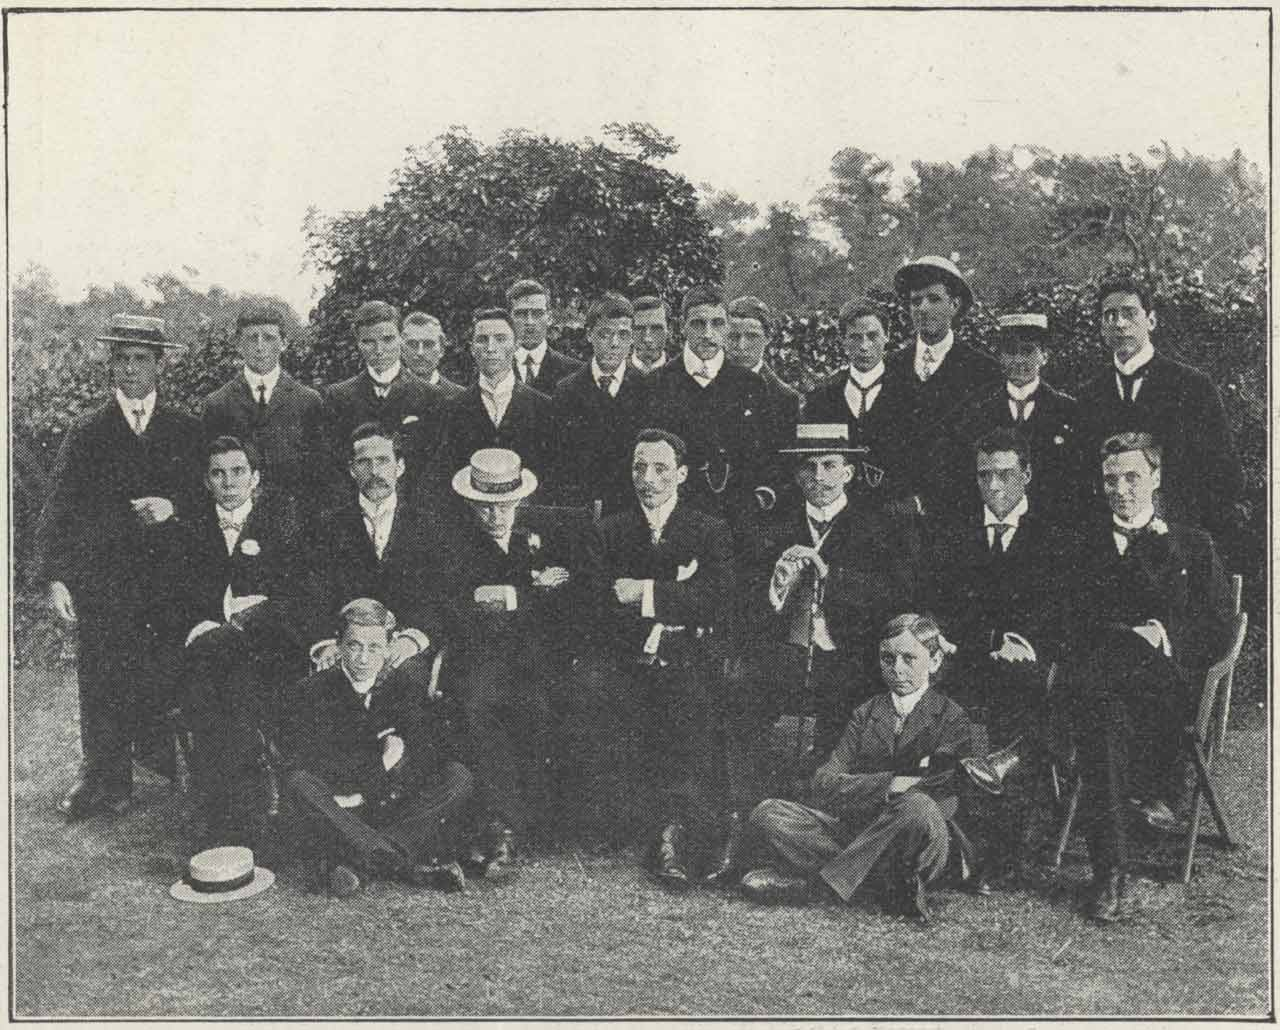
\includegraphics[width=\textwidth]{figures/photo/Greenwich-Observatory-computing-staff-1902.jpg}
      \end{figure}
    \end{column}
    
    \begin{column}{0.4\textwidth}
      \begin{itemize}
        \item Employed computers
        \item 13--20 years old
        \item Overworked
        \item Underpaid
        \item Could be fired at will
      \end{itemize}
    \end{column}
    \end{columns}

\end{frame}


\begin{frame}{George Airy --- whiz kid}
    Airy built complexity into the process, assigning \textit{human computers} 
    to compute, verify, and correct the right ascension and declination of stars.

    \begin{figure}
    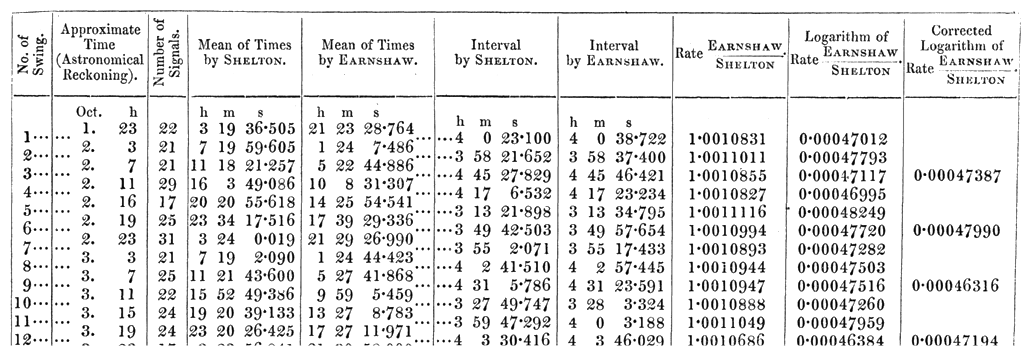
\includegraphics[width=\textwidth]{figures/complexity/pw_literature/airy.png}
    \end{figure}
\end{frame}

\begin{frame}{Cottage Industry}
  % First appearances of piecework:
% \visible<2->{farms}%
% \visible<3->{, textiles}%
% \visible<4->{, and matchsticks.}
  \begin{columns}
  \visible<1->{
    \begin{column}{0.33\textwidth}
    \centering
    Farms
    \begin{figure}
    
\includegraphics[width=\textwidth]{figures/idk.png}
    \end{figure}
    \end{column}
    }
  
  \visible<2->{
  \begin{column}{0.33\textwidth}
  \centering
    Textiles
  \begin{figure}
  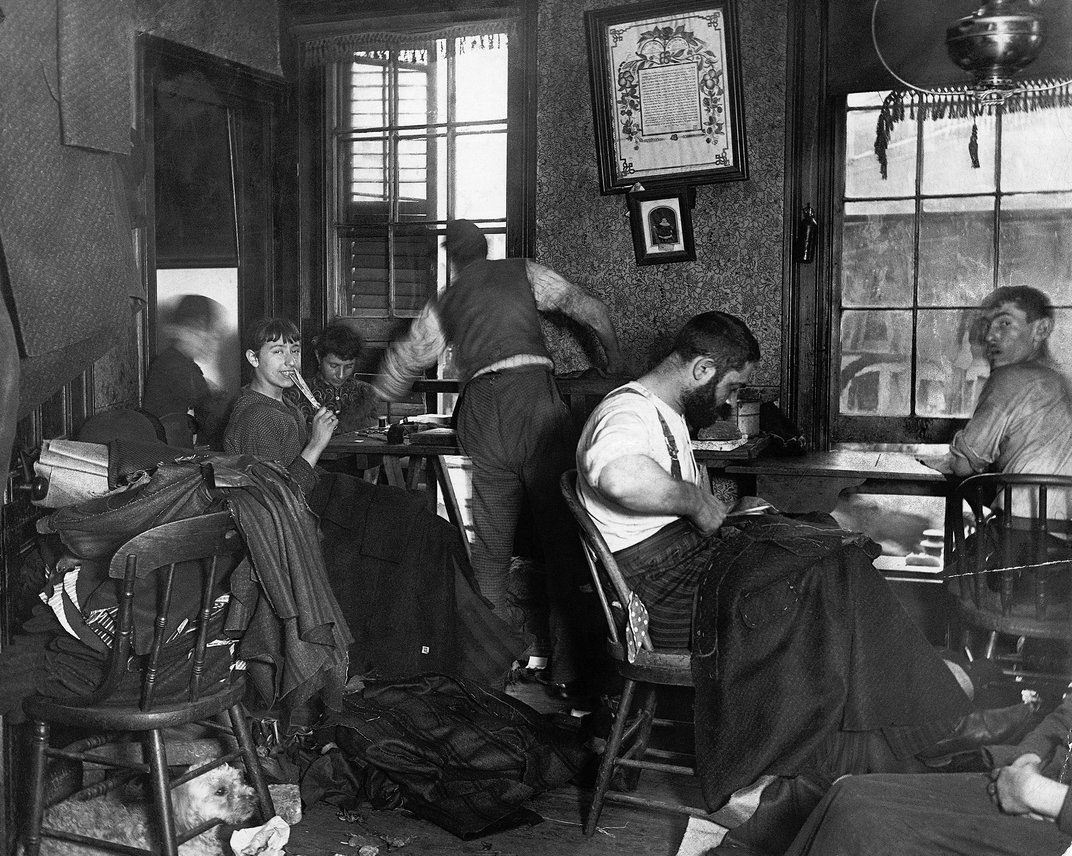
\includegraphics[width=\textwidth]{figures/pieceworkers.jpg}
  \end{figure}
  \end{column}
  }
  
  \visible<3->{
  \begin{column}{0.33\textwidth}
  \centering
    Matchsticks
  \begin{figure}
  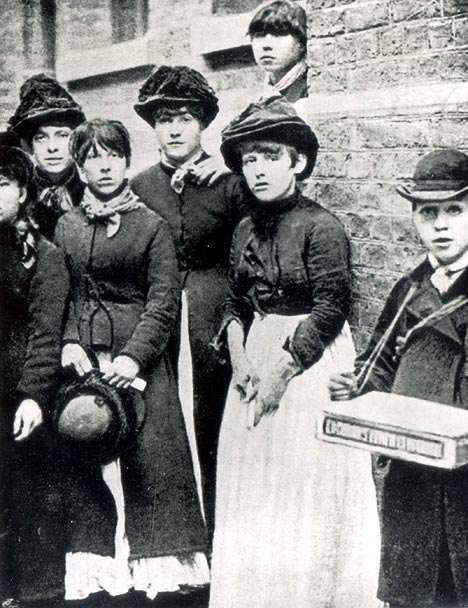
\includegraphics[width=\textwidth]{figures/photo/Matchgirl_strikers.PNG}
  \end{figure}
  \end{column}
  }
  \end{columns}
\end{frame}




\begin{frame}\frametitle{Planes, trains, and automobiles}
             \framesubtitle{{\dots~not in that order}}

  \begin{columns}
  % \vspace{1mm}
  \only<1,4->{
  \begin{column}{0.33\textwidth}
  \centering
  Trains
  \begin{figure}
    \begin{overlayarea}{\textwidth}{4cm}
    \begin{minipage}[c][4cm]{\textwidth}
      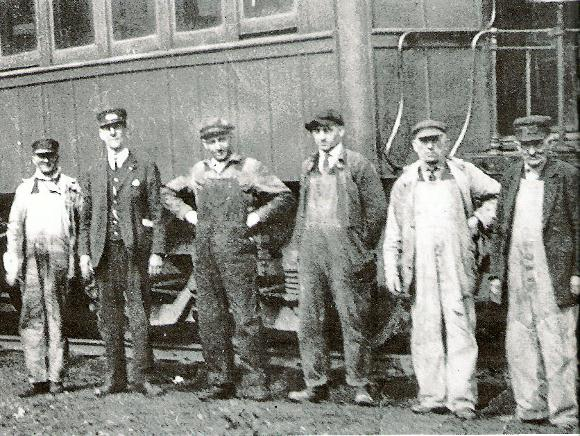
\includegraphics[width=\textwidth]{figures/photo/train_workers.jpg}
    \end{minipage}
    \end{overlayarea}
    % \caption{i wanna fly the train}
    \end{figure}
\end{column}

\only<1>{
    \begin{column}{0.66\textwidth}
      \begin{itemize}
        \item ``Efficiency experts'' measured how long it would take to do various jobs~\cite{doi:10.2307/1883615}
        \item These measurements would be used to assign values for each specific task~\cite{american1921problem}
        \item Train engineers instituted ``The Fix'' to correct perceived unfairness~\cite{roy1954efficiency}
      \end{itemize}
    \end{column}
  }
}

  \only<2,4->{
    \only<2>{
      \begin{column}{0.33\textwidth}
      \begin{itemize}
        \item Fordism, Taylorism, and Scientific Management in full force
      \end{itemize}
      \end{column}
    }

  \begin{column}{0.33\textwidth}
    \centering
      Automobiles
      \begin{figure}
        \begin{overlayarea}{\textwidth}{4cm}
        \begin{minipage}[c][4cm]{\textwidth}
          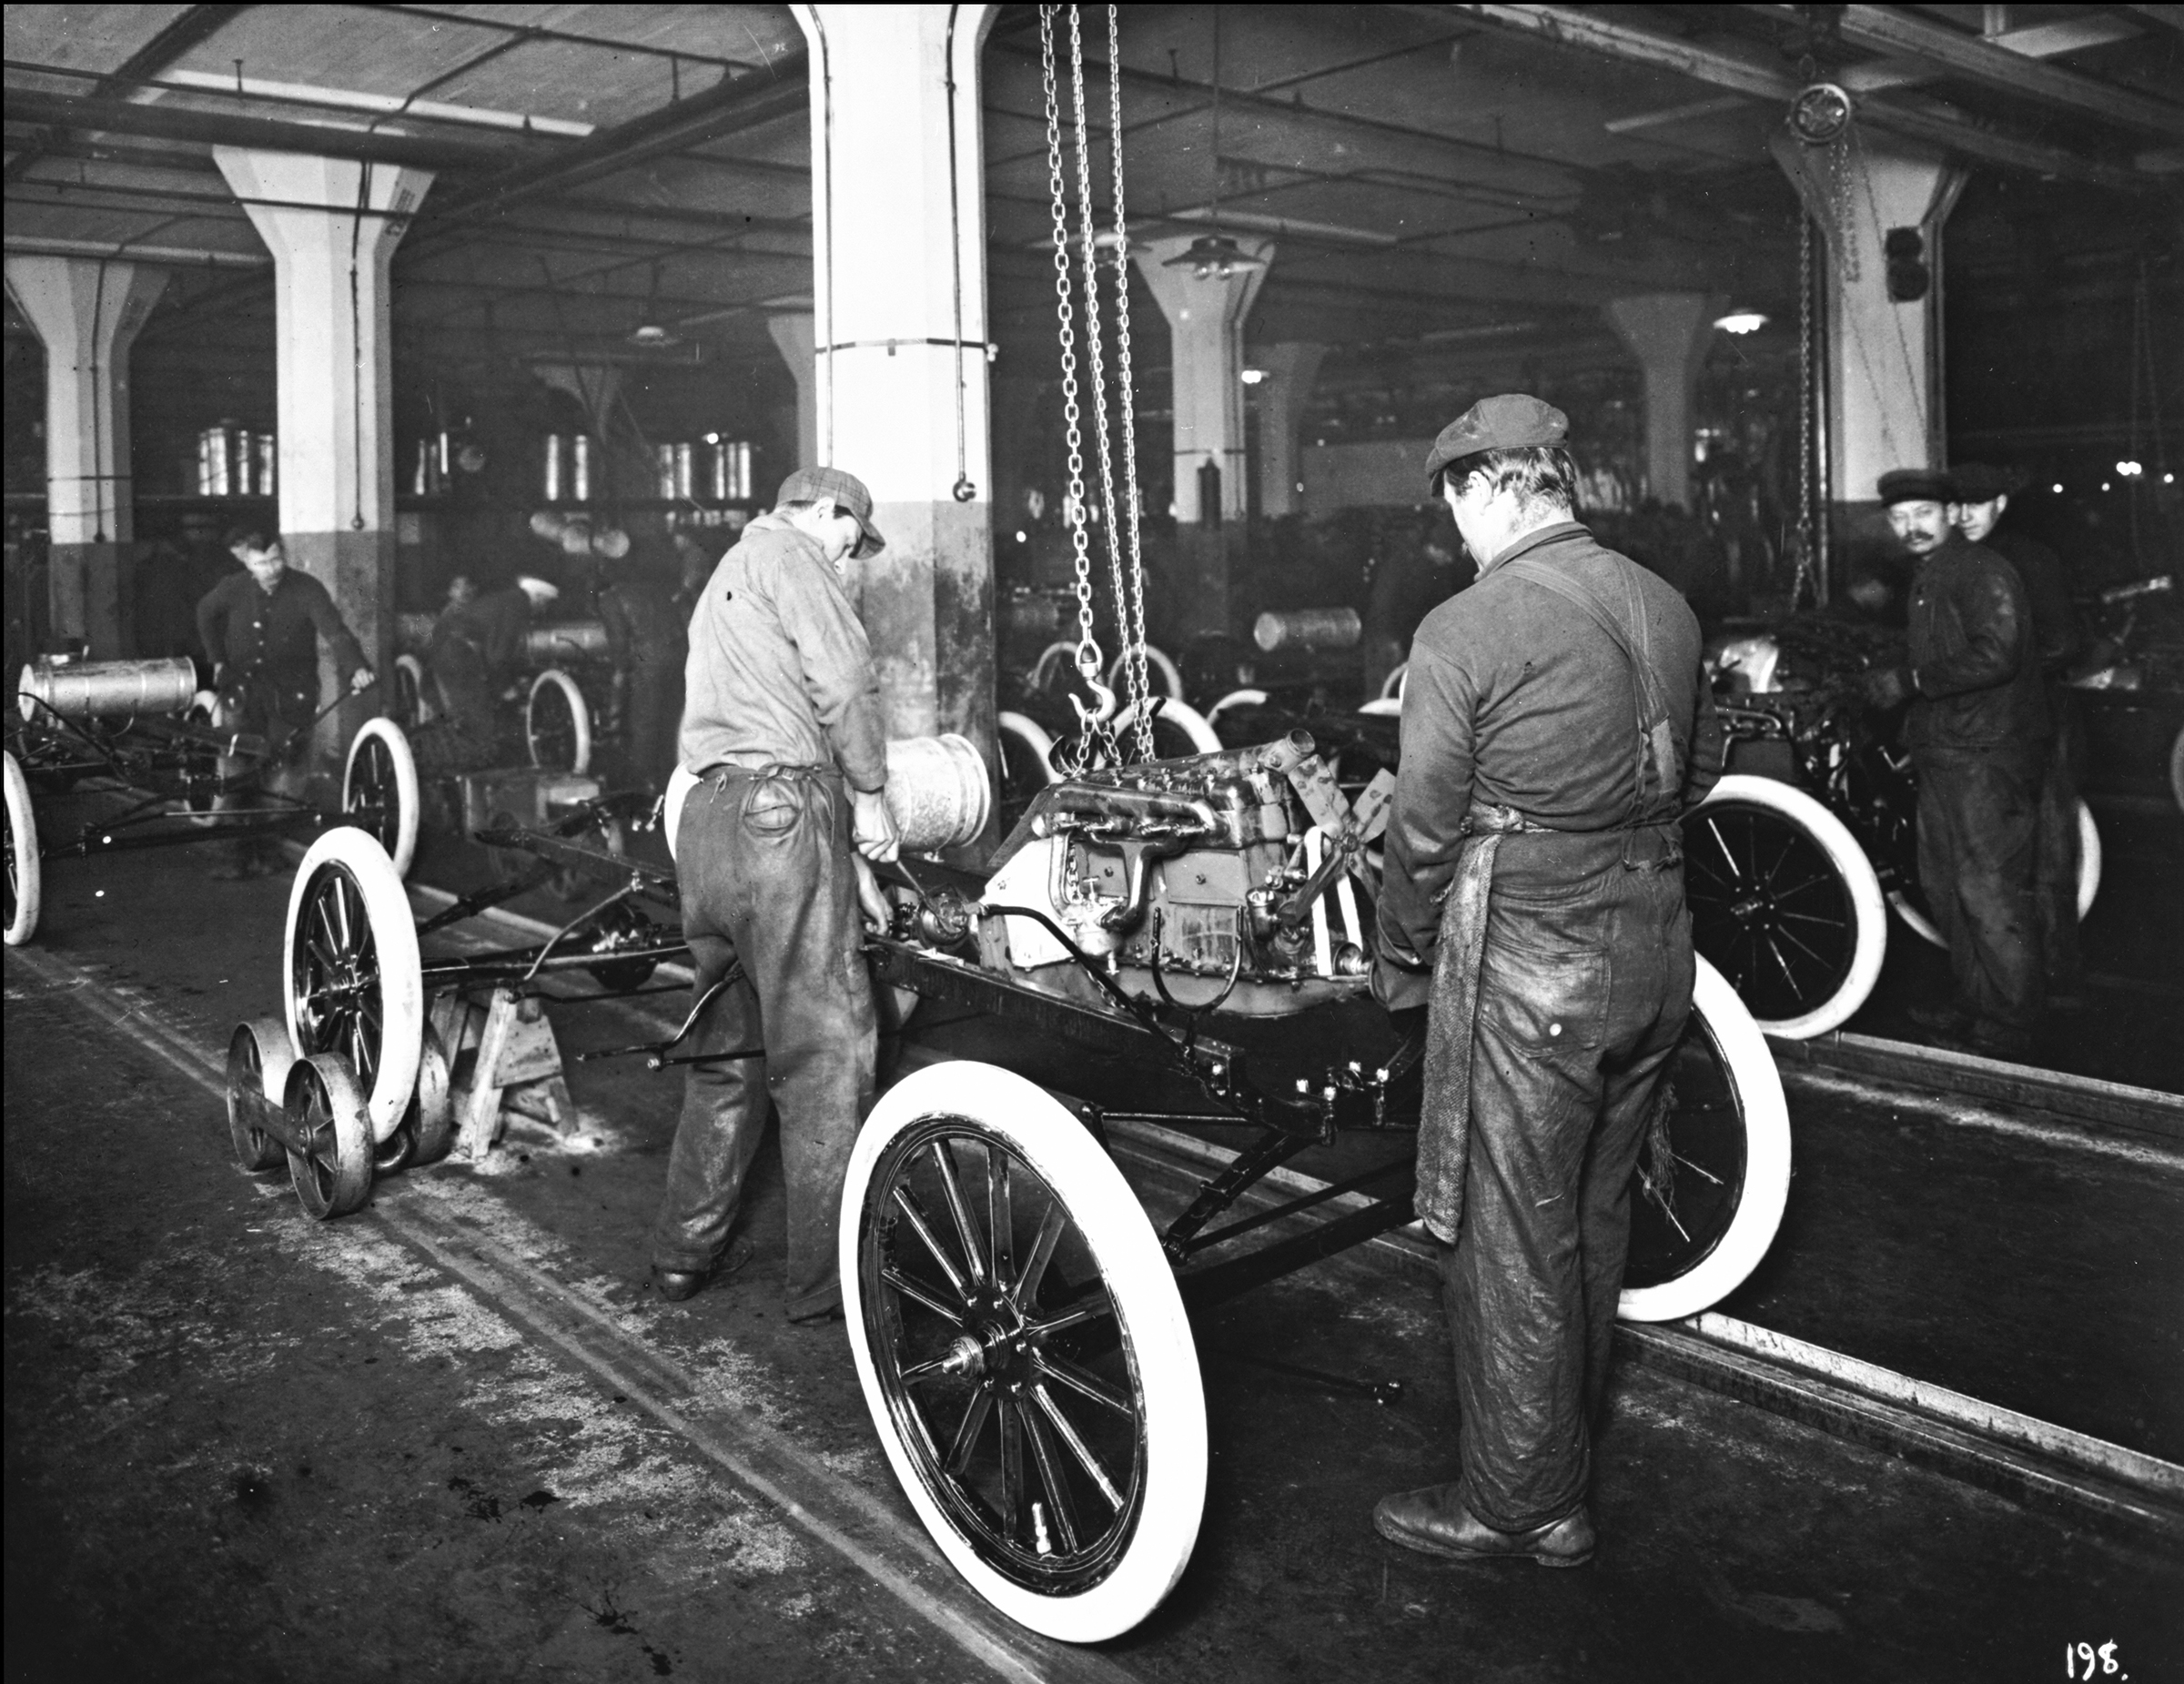
\includegraphics[width=\textwidth]{figures/photo/ford_assembly_line.jpg}
        \end{minipage}
        \end{overlayarea}
        % \caption{something something}
      \end{figure}
  \end{column}
  
  \only<2>{
    \begin{column}{0.33\textwidth}
    \begin{itemize}
      \item \textit{Manufacturing} proved amenable
            to assembly line processes.
    \end{itemize}
    \end{column}
  }
}

  \only<3->{
    \only<3>{
      \begin{column}{0.66\textwidth}
      \end{column}
    }
  \begin{column}{0.33\textwidth}
    \centering
      Planes
      \begin{figure}
        \begin{overlayarea}{\textwidth}{4cm}
        \begin{minipage}[c][4cm]{\textwidth}
            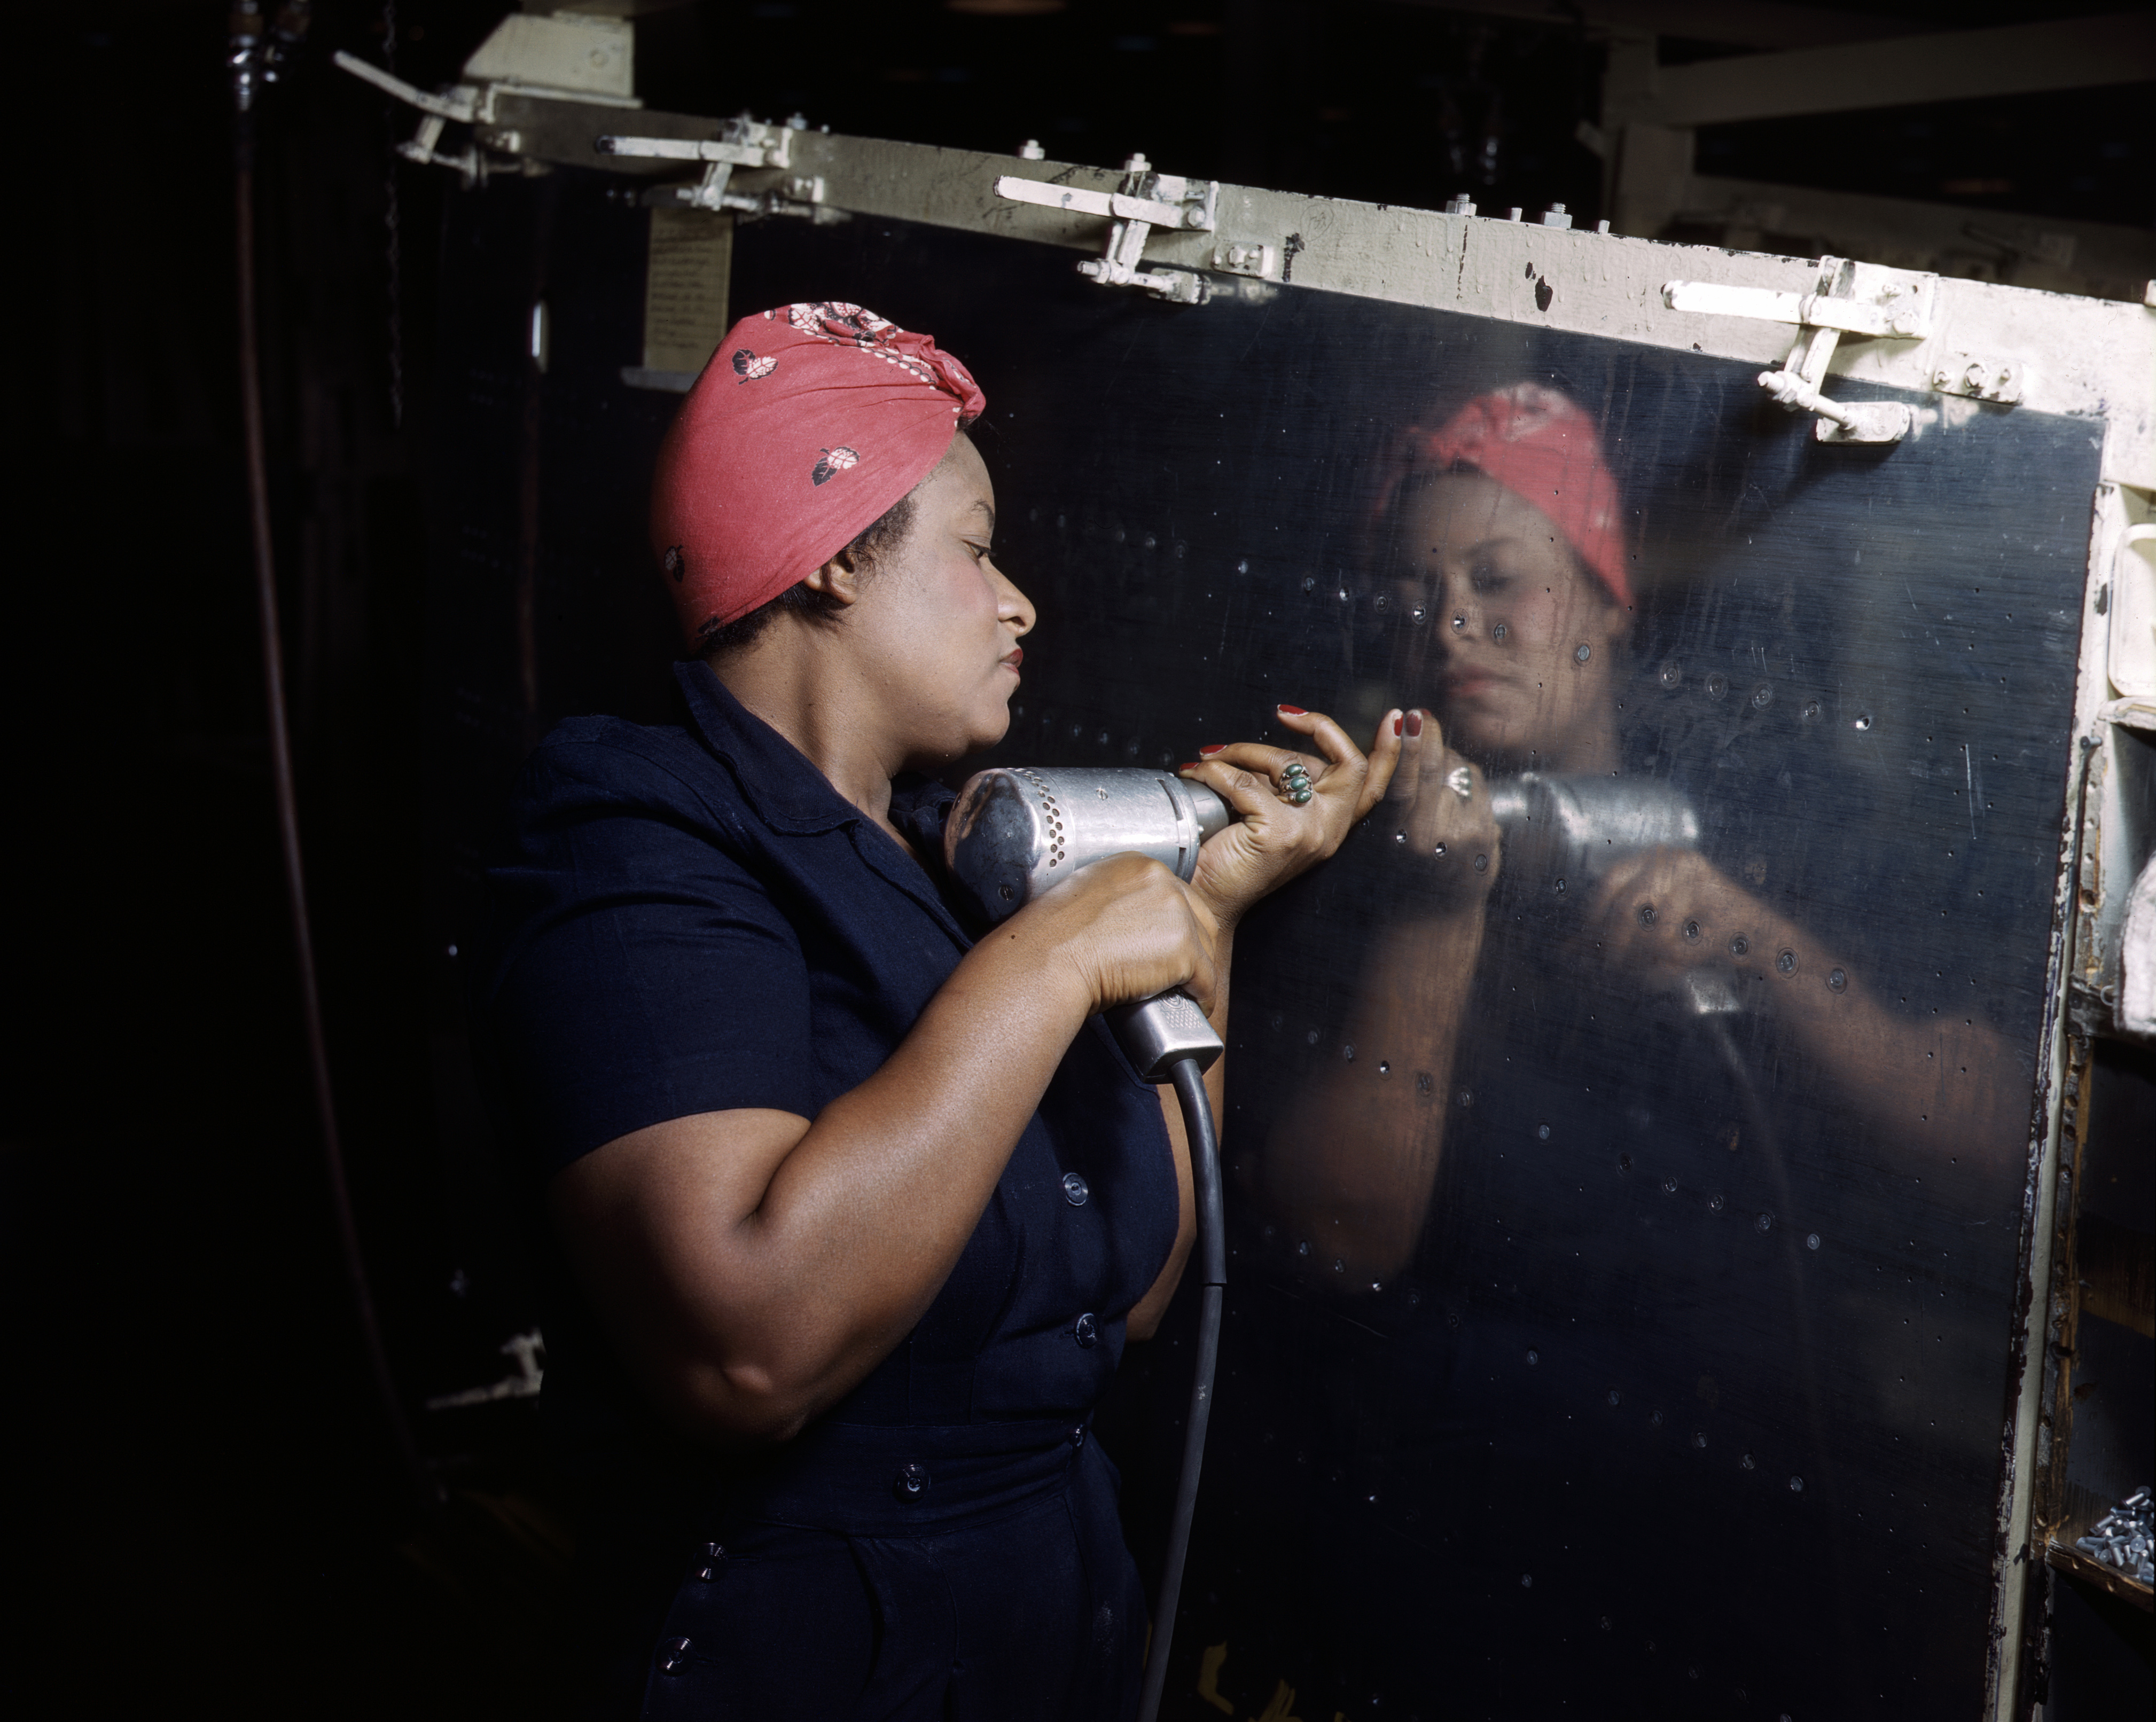
\includegraphics[width=\textwidth]{figures/photo/Rosie_the_Riveter_(Vultee)_DS.jpg}
      \end{minipage}
      \end{overlayarea}
      % \caption{i wanna fly the plane}
      \end{figure}
  \end{column}
  }

  \end{columns}


\end{frame}


\begin{frame}{Comparisons}
\begin{itemize}
  \item Limited array of tasks versus arbitrarily complex work
  \begin{itemize}
    \item \textit{Building} planes versus \textit{fixing} trains
  \end{itemize}
  \item \normalsize{Has technology changed this?}
    \begin{itemize}
      \item Technology makes complex tasks relatively trivial
      \item Measuring workers is easier than ever
    \end{itemize}
\end{itemize}
\end{frame}

\begin{frame}{Complexity}{Cab Drivers}
% \begin{columns}
  % \begin{column}{0.20\textwidth}
    % \begin{itemize}
    %   \item 
      % Cab drivers
    % \end{itemize}
  % \end{column}
  
  % \begin{column}{0.80\textwidth}
  \begin{figure}
  \includegraphics<1>[width=\textwidth]{figures/photo/knowledge-student.jpg}
  \includegraphics<2>[width=\textwidth]{figures/photo/gps-map.jpg}

  \end{figure}
  % \end{column}
% \end{columns}
\end{frame}

\begin{frame}{Complexity}{Algorithmic Measurement}
    notes
    \begin{itemize}
      \item I'm thinking of pointing to UpWork's screen recording tool as a way to measure workers
      \item also maybe google analytics and other ways of tracking web--based workers
    \end{itemize}
\end{frame}

\begin{frame}{Implications}
  \begin{itemize}
    \item We make stronger assumptions about workers' abilities thanks to technology
    \item Evaluation remains difficult, but we're trying to find stopgap solutions through decomposition
    \item We're still not solving the problems of inherently subjectively judged work
  \end{itemize}
\end{frame}

\onlyinsubfile{
  \printbibliography{}
}
\end{document}